
\section{Dati d'esempio}

	Esistono 6 file di dati d'esempio che prendono le immagini da 3 set distinti; a coppie, i file richiedono la soluzione su uno stesso set di immagini, ma con parametri diversi. \\
	Per ogni set vengono presentati i dati distinti con i parametri utilizzati nei relativi file. Quindi si mostrerà l'output del programma \texttt{amplide} seguito dai valori delle variabili della soluzione. \\
	La soluzione si compone del valore della funzione obiettivo, che coincide con la variabile D, seguito da una tupla nel formato <nome, X, Y, larghezza, altezza, rotazione> per ogni immagine. \\
	Seguirà poi un confronto grafico tra le soluzioni dei vari problemi con parametri diversi.


%%%%%%%%%%
%% SET 1
%%%%%%%%%%

	\subsection{Set 1}
	%\subsubsection{Immagini}
\iffalse
	Nel set sono presenti 6 immagini:
	\begin{itemize}
		\itemsep0em
		\item \texttt{a:\ 16x16};
		\item \texttt{b:\ \ 8x16};
		\item \texttt{c:\ \ 8x\ 8};
		\item \texttt{d:\ \ 5x25};
		\item \texttt{e:\ 72x32};
		\item \texttt{f:\ 32x32};
	\end{itemize}
\fi
%
Dati del set di immagini:  \\
%

\begin{table}[h!]
\centering
\footnotesize
\begin{tabular}{l|r|r}
\multicolumn{3}{c}{\textbf{Immagini}} \\ 
%\hline
id & larghezza & altezza \\
\hline
a & 16 & 16 \\
		 b & 8&16\\
		 c & 8& 8\\
		 d & 5&25\\
		 e & 72&32\\
		 f & 32 &32\\
\end{tabular}
\end{table}
%
%\subsubsection{Risultati}


\noindent Parametri, Output e Soluzione dei 2 problemi: 

\begin{table}[h]
\centering
\footnotesize
\begin{tabular}{p{5cm}|p{5cm}}
%\hline
\textbf{Problema 1} & \textbf{Problema 2} \\
\hline
\multicolumn{2}{|c|}{Parametri} \\ 
\hline
allowRotations = 0,\newline
useNoBleeding = 0,\newline
usePowersOf2 = 1;	& 
allowRotations = 1,\newline
useNoBleeding = 1,\newline
usePowersOf2 = 1;	\\
\hline
\multicolumn{2}{|c|}{Output AMPL} \\
\hline
\texttt{69 MIP simplex iterations \newline
0 branch-and-bound nodes \newline
D = 128}
&
\texttt{69 MIP simplex iterations \newline
0 branch-and-bound nodes \newline
D = 128}
\\
\hline
\multicolumn{2}{|c|}{Soluzione} \\
\hline
\texttt{128 \newline
109,1,16,16,0\newline
37,0,8,16,0\newline
0,0,8,8,0\newline
32,0,5,25,0\newline
37,16,72,22,0\newline
0,8,32,32,0}
&
\texttt{128 \newline
109,1,16,16,0\newline
37,0,8,16,0\newline
0,0,8,8,0\newline
32,0,5,25,0\newline
37,16,72,22,0\newline
0,8,32,32,0}
\\
   \hline
\end{tabular}
\end{table}

	%\subsubsection{Risultati}



















%%%%%%%%%%
%% SET 2
%%%%%%%%%%

	\subsection{Set 1}
	%\subsubsection{Immagini}
\iffalse
	Nel set sono presenti 6 immagini:
	\begin{itemize}
		\itemsep0em
		\item \texttt{a:\ 16x16};
		\item \texttt{b:\ \ 8x16};
		\item \texttt{c:\ \ 8x\ 8};
		\item \texttt{d:\ \ 5x25};
		\item \texttt{e:\ 72x32};
		\item \texttt{f:\ 32x32};
	\end{itemize}
\fi
%
Dati del set di immagini:  \\
%

\begin{table}[h!]
\centering
\footnotesize
\begin{tabular}{l|r|r}
\multicolumn{3}{c}{\textbf{Immagini}} \\ 
%\hline
id & larghezza & altezza \\
\hline
a & 16 & 16 \\
		 b & 8&16\\
		 c & 8& 8\\
		 d & 5&25\\
		 e & 72&32\\
		 f & 32 &32\\
\end{tabular}
\end{table}
%
%\subsubsection{Risultati}


\noindent Parametri, Output e Soluzione dei 2 problemi: 

\begin{table}[h]
\centering
\footnotesize
\begin{tabular}{p{5cm}|p{5cm}}
%\hline
\textbf{Problema 1} & \textbf{Problema 2} \\
\hline
\multicolumn{2}{|c|}{Parametri} \\ 
\hline
allowRotations = 0,\newline
useNoBleeding = 0,\newline
usePowersOf2 = 1;	& 
allowRotations = 1,\newline
useNoBleeding = 1,\newline
usePowersOf2 = 1;	\\
\hline
\multicolumn{2}{|c|}{Output AMPL} \\
\hline
\texttt{69 MIP simplex iterations \newline
0 branch-and-bound nodes \newline
D = 128}
&
\texttt{69 MIP simplex iterations \newline
0 branch-and-bound nodes \newline
D = 128}
\\
\hline
\multicolumn{2}{|c|}{Soluzione} \\
\hline
\texttt{128 \newline
109,1,16,16,0\newline
37,0,8,16,0\newline
0,0,8,8,0\newline
32,0,5,25,0\newline
37,16,72,22,0\newline
0,8,32,32,0}
&
\texttt{128 \newline
109,1,16,16,0\newline
37,0,8,16,0\newline
0,0,8,8,0\newline
32,0,5,25,0\newline
37,16,72,22,0\newline
0,8,32,32,0}
\\
   \hline
\end{tabular}
\end{table}

	%\subsubsection{Risultati}






%%%%%%%%%%
%% SET 3
%%%%%%%%%%

	\subsection{Set 1}
	%\subsubsection{Immagini}
\iffalse
	Nel set sono presenti 6 immagini:
	\begin{itemize}
		\itemsep0em
		\item \texttt{a:\ 16x16};
		\item \texttt{b:\ \ 8x16};
		\item \texttt{c:\ \ 8x\ 8};
		\item \texttt{d:\ \ 5x25};
		\item \texttt{e:\ 72x32};
		\item \texttt{f:\ 32x32};
	\end{itemize}
\fi
%
Dati del set di immagini:  \\
%

\begin{table}[h!]
\centering
\footnotesize
\begin{tabular}{l|r|r}
\multicolumn{3}{c}{\textbf{Immagini}} \\ 
%\hline
id & larghezza & altezza \\
\hline
a & 16 & 16 \\
		 b & 8&16\\
		 c & 8& 8\\
		 d & 5&25\\
		 e & 72&32\\
		 f & 32 &32\\
\end{tabular}
\end{table}
%
%\subsubsection{Risultati}


\noindent Parametri, Output e Soluzione dei 2 problemi: 

\begin{table}[h]
\centering
\footnotesize
\begin{tabular}{p{5cm}|p{5cm}}
%\hline
\textbf{Problema 1} & \textbf{Problema 2} \\
\hline
\multicolumn{2}{|c|}{Parametri} \\ 
\hline
allowRotations = 0,\newline
useNoBleeding = 0,\newline
usePowersOf2 = 1;	& 
allowRotations = 1,\newline
useNoBleeding = 1,\newline
usePowersOf2 = 1;	\\
\hline
\multicolumn{2}{|c|}{Output AMPL} \\
\hline
\texttt{69 MIP simplex iterations \newline
0 branch-and-bound nodes \newline
D = 128}
&
\texttt{69 MIP simplex iterations \newline
0 branch-and-bound nodes \newline
D = 128}
\\
\hline
\multicolumn{2}{|c|}{Soluzione} \\
\hline
\texttt{128 \newline
109,1,16,16,0\newline
37,0,8,16,0\newline
0,0,8,8,0\newline
32,0,5,25,0\newline
37,16,72,22,0\newline
0,8,32,32,0}
&
\texttt{128 \newline
109,1,16,16,0\newline
37,0,8,16,0\newline
0,0,8,8,0\newline
32,0,5,25,0\newline
37,16,72,22,0\newline
0,8,32,32,0}
\\
   \hline
\end{tabular}
\end{table}

	%\subsubsection{Risultati}



\newpage

\subsection{Confronti grafici}

%\begin{figure}[h!]
% \noindent Confronto grafico: \\
Di seguito le immagini ottenute dalle soluzioni dei due problemi. \\
In sequenza, da sinistra a destra, dall'alto al basso, le immagini rispettivamente del Problema 1, 2, 3, 4, 5, 6. \\
 In ogni immagine, per ogni texture del texture atlas viene utilizzato un colore diverso; il contorno bianco indica l'eventuale bordo necessario per evitare l'effetto bleeding. 
	 %A sinistra il 1\degree{} problema, a destra il 2\degree. \\
\subsubsection{Problemi 1 e 2}
\vcenter{
\centering
	
\includegraphics[width=5cm]{results01}
	\hspace{1cm}
	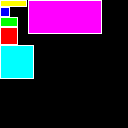
\includegraphics[width=5cm]{results02}
}\\
\subsubsection{Problemi 3 e 4}
\vcenter{
\centering
	
\includegraphics[width=5cm]{results01}
	\hspace{1cm}
	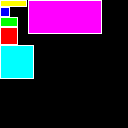
\includegraphics[width=5cm]{results02}
} \\
\subsubsection{Problemi 5 e 6}
\vcenter{
\centering
	
\includegraphics[width=5cm]{results01}
	\hspace{1cm}
	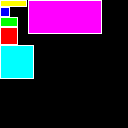
\includegraphics[width=5cm]{results02}
}




\iffalse
\newpage
{\centering
	
\includegraphics[width=4cm]{results01}
	\hspace{1cm}
	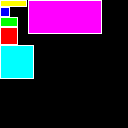
\includegraphics[width=4cm]{results02}
	\caption{\\Le immagini ottenute dalle soluzioni dei due problemi. 
	 A sinistra il 1\degree{} problema, a destra il 2\degree. \\
	 { %\footnotesize
	 Per ogni immagine viene utilizzato un colore diverso; il contorno bianco indica il bordo necessario per evitare l'effetto bleeding.
	 } } }
%\end{figure}
\begin{figure}[h!]
% \noindent Confronto grafico: \\
{\centering
	
\includegraphics[width=4cm]{results01}
	\hspace{1cm}
	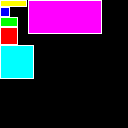
\includegraphics[width=4cm]{results02}
	\caption{\\Le immagini ottenute dalle soluzioni dei due problemi. 
	 A sinistra il 1\degree{} problema, a destra il 2\degree. \\
	 { %\footnotesize
	 Per ogni immagine viene utilizzato un colore diverso; il contorno bianco indica il bordo necessario per evitare l'effetto bleeding.
	 } } }
\end{figure}


\begin{figure}[h!]
% \noindent Confronto grafico: \\
{\centering
	
\includegraphics[width=4cm]{results01}
	\hspace{1cm}
	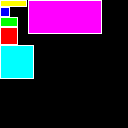
\includegraphics[width=4cm]{results02}
	\caption{\\Le immagini ottenute dalle soluzioni dei due problemi. 
	 A sinistra il 1\degree{} problema, a destra il 2\degree. \\
	 { %\footnotesize
	 Per ogni immagine viene utilizzato un colore diverso; il contorno bianco indica il bordo necessario per evitare l'effetto bleeding.
	 } } }
\end{figure}


\fi






\iffalse

ampl: include atlas.run;
CPLEX 12.6.3.0: optimal integer solution; objective 128
69 MIP simplex iterations
0 branch-and-bound nodes
No basis.
D = 128

ampl: include atlas.run;
CPLEX 12.6.3.0: optimal integer solution; objective 128
110 MIP simplex iterations
0 branch-and-bound nodes
No basis.
D = 128

ampl: include atlas.run;
CPLEX 12.6.3.0: optimal integer solution; objective 228
16295 MIP simplex iterations
2405 branch-and-bound nodes
No basis.
D = 228

ampl: include atlas.run;
CPLEX 12.6.3.0: optimal integer solution; objective 224
1084 MIP simplex iterations
277 branch-and-bound nodes
No basis.
D = 224

ampl: include atlas.run;
CPLEX 12.6.3.0: optimal integer solution; objective 198
4403 MIP simplex iterations
1423 branch-and-bound nodes
No basis.
D = 198

ampl: include atlas.run;
CPLEX 12.6.3.0: optimal integer solution; objective 256
222 MIP simplex iterations
0 branch-and-bound nodes
No basis.
D = 256
























128,0
109,1,16,16,0
37,0,8,16,0
0,0,8,8,0
32,0,5,25,0
37,16,72,22,0
0,8,32,32,0

128,1
0,27,18,18,0
0,17,18,10,1
0,7,10,10,0
0,0,27,7,1
28,4,74,24,0
0,45,34,34,0

228,1
98,0,130,34,0
194,100,34,34,0
132,34,66,66,0
132,100,34,98,1
194,134,34,66,0
98,58,34,170,1
0,98,98,130,0
0,0,98,98,0

224,0
32,0,128,32,0
192,0,32,32,0
96,64,64,64,0
0,192,96,32,0
0,0,32,64,0
56,32,168,32,0
0,64,96,128,0
97,128,96,96,0

198,1
180,0,18,34,0
164,164,34,34,0
170,0,10,10,0
169,83,7,17,0
136,0,34,66,0
0,0,34,170,1
34,100,130,98,1
34,0,98,98,0

256,1
98,0,18,34,0
10,0,34,34,0
0,0,10,10,0
0,17,7,17,0
0,170,34,66,0
116,0,34,170,1
158,0,98,130,0
0,34,98,98,0


\fi











	\newpage

